\subsubsection*{Transfer to population ratio}
  If immigrants are responsible for a relatively small share of public transfers compared to natives, they appear to account for a disproportionate share in regard to their population share (\autoref{tab:tx2015}).
In 2015 for instance, immigrants represent about 24.2\% of the Canadian population but contribute to only 22.7\% of outflows.
Furthermore, while their share in inflow transfers (25.2\% ) is much closer to their share in the population, there is a significant gap between inflows sub-accounts.
For instance, immigrants are only responsible for 14.5\% of education costs but account for 29.5\% for health expenses.
For outflow accounts, the share ranges from 21.7\% for sales taxes at one end and 25.4\% for social insurance contributions at the other end.
In dollar values, net transfer to public finances in 2015 is positive (19 004 million or 0.96\% of GDP) for immigrants but slightly negative (7 120 million \$ or 0.36\% of GDP) for natives.
However, as the benefits of immigrations become visible only in the medium and long term (Goldin et al., 2011), a more accurate analysis requires a comparison over many years.

  \begin{table}[H]%
    \caption{Population and aggregates public transfers, Canada 2015}
    \label{tab:tx2015}%
    \begin{center}
      \resizebox{1\textwidth}{!}{%
      \begin{threeparttable}
        %latex.default(tab2015, file = file.path(path, "Docs/ntaImmig/res/tab2015.tex"),     booktabs = TRUE, collabel.just = c("l", "r", "r", "r", "r",         "r"), col.just = c("l", "r", "r", "r", "r", "r"), center = "none",     rowname = NULL, table.env = FALSE, longtable = FALSE, cgroup = c("",         "Absolute numbers", "Percentage"), n.cgroup = c(1, 3,         2), dcolumn = TRUE, )%
\newcolumntype{.}{D{.}{.}{-1}}
\begin{tabular}{lcD{.}{.}{-1}rrcD{.}{.}{-1}D{.}{.}{-1}}
\toprule
\multicolumn{1}{c}{\bfseries }&\multicolumn{1}{c}{\bfseries }&\multicolumn{3}{c}{\bfseries Absolute numbers}&\multicolumn{1}{c}{\bfseries }&\multicolumn{2}{c}{\bfseries Percentage}\tabularnewline
\cline{3-5} \cline{7-8}
\multicolumn{1}{l}{Items}&\multicolumn{1}{c}{}&\multicolumn{1}{r}{Canada}&\multicolumn{1}{r}{Natives}&\multicolumn{1}{r}{Immigrants}&\multicolumn{1}{c}{}&\multicolumn{1}{r}{Natives}&\multicolumn{1}{r}{Immigrants}\tabularnewline
\midrule
\textbf{Population}&&~35065&26575&8490&&~75.8&~24.2\tabularnewline
&&&&&&&\tabularnewline
\textbf{Inflows Transfers}&&638972&478204&160768&&~74.8&~25.2\tabularnewline
\quad Cash transfers (Cash)&&228722&165925&62797&&~72.5&~27.5\tabularnewline
\quad Education Cost (Education)&&~97209&83130&14079&&~85.5&~14.5\tabularnewline
\quad Health Expenses (Health)&&154292&108837&45455&&~70.5&~29.5\tabularnewline
\quad Other Inflows (Others)&&158749&120312&38437&&~75.8&~24.2\tabularnewline
\quad &&&&&&&\tabularnewline
\textbf{Outflows Transfers}&&627472&485325&142147&&~77.3&~22.7\tabularnewline
\quad Contributions to social insurance plans (Insurance)&&~93238&69580&23658&&~74.6&~25.4\tabularnewline
\quad Taxes on Products and Imports (Sales)&&235613&184420&51193&&~78.3&~21.7\tabularnewline
\quad Person Income Taxes (Income)&&238391&186447&51944&&~78.2&~21.8\tabularnewline
\quad Corporate Taxes (Business)&&~68197&51040&17157&&~74.8&~25.2\tabularnewline
\quad Other Outflows (Others)&&~-7968&-6163&-1805&&~77.3&~22.7\tabularnewline
\quad &&&&&&&\tabularnewline
\textbf{Inflows minus Outflows (Net Transfer)}&&~11500&-7120&18620&&-61.9&161.9\tabularnewline
\bottomrule
\end{tabular}
%
        \begin{tablenotes}
          \small
          \item [.] values are in millions \$
          \item [.] Source: Authors Calculations
       \end{tablenotes}
     \end{threeparttable}
      }
   \end{center}
\end{table}%

  While the aggregate Net transfer is positive for immigrants and negative for natives for the year 2015, this trend is relatively recent as it became apparent only from 2012.
\autoref{fig:aggTrend} shows that the opposite trend was prevailing till 2001, with immigrants contributing about 5\% more than their population share.
Between 2002 and 2011, immigrants and native contributed to public finances roughly in the same proportion as their population share.
While the trend in outflows has reversed throughout the study period for the two populations, the trend in inflows has been much stable, especially for natives who received between one and two percent less public transfer than their population share.
For immigrants, the cost was about 10\% more till 2001 but decreased gradually to about 5\% more than their population.
Although aggregate measures provide interesting insights about the relative cost of immigration in Canada, crude values per-capita values are better indicators for comparing immigrants and natives, as they remove the effect of the population size.

  \begin{figure}[H]%
    \caption{Transfer share as a ratio to Population share for Immigrants and Natives between 1997 to 2015}
    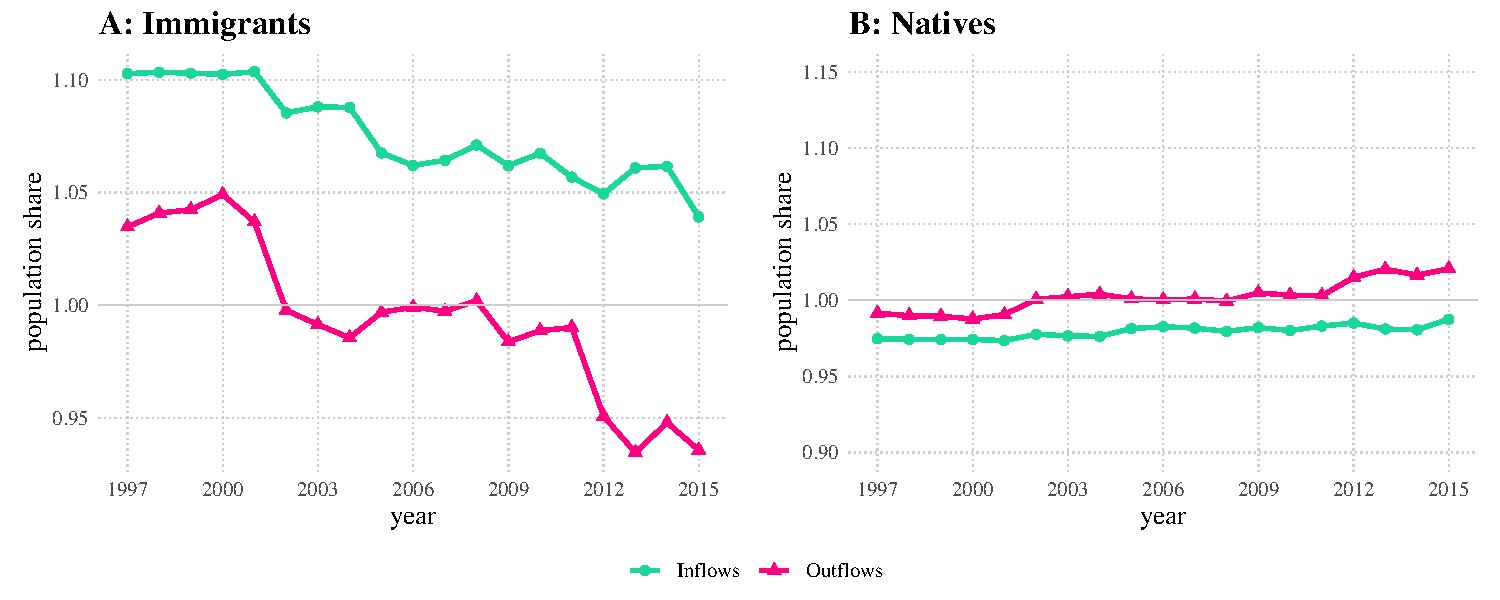
\includegraphics[width=1\textwidth]{res/aggTrend.pdf}%
    \label{fig:aggTrend}%
  \end{figure}%

  \subsubsection*{Net transfers and Immigrant surpluses}

  \autoref{fig:netDiff} shows the trends in Net Surplus as derived from Net Transfers (A) on one hand and Immigrant Surpluses (B) on the other hand between 1997 and 2015.
Excluding the sudden increase from 2011 which increase it to \$\DTLfetch{statex}{sKey}{AveperCapita}{sVal}, the average net surplus of transfer has fluctuated only slightly around \$1400 since 1997.
A positive net surplus of transfer implies that the average immigrant has cost the state more than the average native.
However, this overall positive cost says little about the origins of these costs, as it hides important differences in trends within each group and transfer components.

  \vspace{0.7em}\par
  Looking at the trend in Net transfer (\autoref{fig:netDiff}-A) separately for immigrant and native, it can be observed that Immigrants have had a positive net transfer over the studied period.
This positive net transfer implies that immigrants have consistently received more transfers from the state than they contribute to its revenues.
Between 1997 and 2011, the average net transfer for immigrants fluctuated around \$1400 per year.
However, it rose rapidly between 2011 and 2013 to surpass \$2100.
Although at a much lower level, natives have also seen a positive Net transfer between 1997 and 2002.
However, net transfer among native drops and become negative since 2003.
Between 2005 and 2015, net transfer among natives has mostly been negative with slight fluctuation around \$280, a sign that they contribute more to the public purse than they received from it.

  \begin{figure}[H]%
    \caption{Difference in Inflows and Outflows transfers for Immigrant and Natives between 1997 to 2015}
    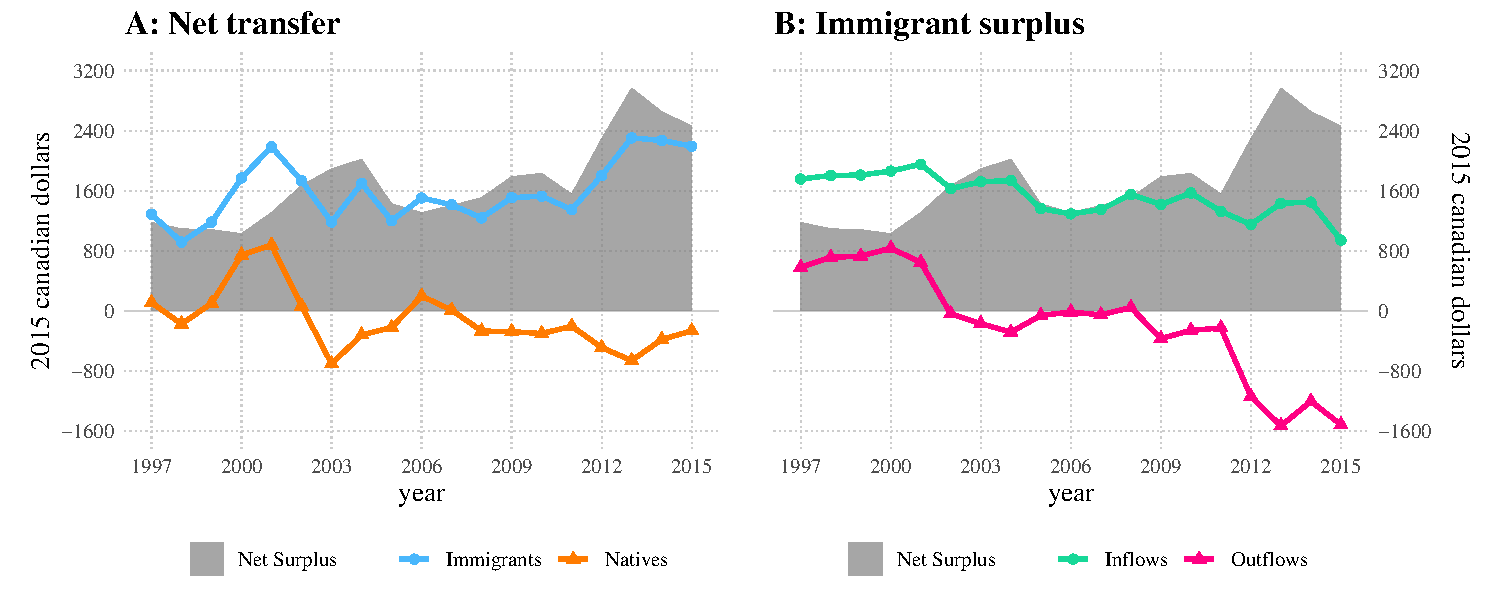
\includegraphics[width=1\textwidth]{res/netDiff.pdf}%
    \label{fig:netDiff}%
\end{figure}%

  \vspace{0.7em}\par
  Putting these observations together it can be concluded that the positive net surplus and its stability between 1997 and 2011 is because immigrants have consistently received more than they contributed while natives have received slightly less than they contributed.
But, it is still unclear how inflows and outflows have trended during the studied period and to which one can be attributed the sudden increase in the net surplus of transfer from 2012.
These differences can be further understood by analyzing the trend in Immigrant surplus for each transfer components (\autoref{fig:netDiff}-B ).

  \vspace{0.7em}\par
  Over the studied period, the Immigrant surplus for inflow has been positive, with immigrants receiving about \$1400 more than natives on average.
It can also be observed that transfers to immigrants have been slowing down compared to natives.
For instance, the Immigrant surplus for inflow has dropped by about \$700 between 1997 and 2015 and if the surplus for outflows were maintained at its early 2000s level, the net surplus of transfer between immigrants and natives would be close to null by 2015.
Instead, while the surplus for inflow decreased slowly and steadily, the surplus for outflow increased drastically between 1997 and 2015.
For instance, before 2002 the average immigrant contributes about \$700 more than native in outflow transfer.
From early 2000 however, the surplus in outflow dropped significantly and between 2002 and 2008, both immigrants and natives contribute about the same amount.
The situation reverses between 2009 and 2011 with immigrants contributing slightly less than natives.
From 2012 however, the gap in outflow transfer deepened with natives contributing about \$1400 more than immigrants.

  \vspace{0.7em}\par
  Although Net transfer and Net surplus result in the same net surplus, they illustrate different aspects of the transfer dynamic and reveal two important facts.
First, the increase in Net transfer between 2000 and 2004 is mainly due to the increase in native outflows while that of immigrant stagnated.
Second, and contrary to the first point, the increase in net surplus between 2011 and 2013 is caused by a decrease in immigrant's outflows while that of native stagnated.
As outflows are solely dependant on individual labor outcomes, these results suggest that the labor prospect of immigrants has degraded compared to natives during the study period.
However, being based on the crude values of transfers, the results do not account for the difference in the age structure of the two populations.
Therefore, proper isolation of demographic effect is necessary for an unbiased comparison of transfer differences between immigrants and natives.















